\documentclass[a4paper, 6pt, landscape]{scrartcl}
\usepackage[german]{babel}
\usepackage[utf8]{inputenc}
\usepackage{multicol}
\usepackage{geometry}
\usepackage{graphicx}
\usepackage{wrapfig}
\usepackage{enumitem}
\usepackage{fancyhdr}
\usepackage{index}
\usepackage{sectsty}
\usepackage{mwe}
\usepackage{comment}
\usepackage{lipsum}
\usepackage{titlesec}
\usepackage[dvipsnames]{xcolor}
\usepackage{amsmath}
\usepackage{amssymb}
\usepackage{listings}
\usepackage{graphicx}
\usepackage{graphicx}

%Define Math Commands:
\newcommand*{\field}[1]{\mathbb{#1}}%
\newcommand{\Mod}[1]{\ (\mathrm{mod}\ #1)}

%Image Folder:
\graphicspath{{../img/}}

%format
\geometry{top=0.4cm,left=0.5cm,right=0.5cm,bottom=0.4cm}
\setlist{topsep=0pt, leftmargin=5mm, nolistsep}

% Code Snippets

\definecolor{javared}{rgb}{0.6,0,0} % for strings

\lstdefinelanguage{JavaScript}{
keywords={typeof, new, true, false, catch, function, return, null, catch, switch, var, if, in, while, do, else, case, break},
ndkeywords={class, export, boolean, throw, implements, import, this},
ndkeywordstyle=\color{darkgray}\bfseries,
identifierstyle=\color{black},
sensitive=false,
comment=[l]{//},
morestring=[b]',
morestring=[b]"
}

\lstset{
language=JavaScript,
basicstyle=\fontsize{6}{6} \ttfamily,
keywordstyle=\bfseries\color{RoyalBlue},
stringstyle=\color{javared},
commentstyle=\color{MidnightBlue},
morecomment=[s][\color{MidnightBlue}]{/*}{*/},
tabsize=2,
showspaces=false,
showstringspaces=false,
texcl = true,
rulecolor = \color{black},
breaklines = true,
aboveskip = 0em,
belowskip = 0em
}




% Define Section Format
\titleformat{name=\section}[block]
{\sffamily\normalsize}
{}
{0pt}
{\colorsection}
\titlespacing*{\section}{0pt}{0pt}{0pt}

\newcommand{\colorsection}[1]{%
\colorbox{MidnightBlue!40}{\parbox{0.98\linewidth}{\color{black}\thesection\ #1}}}


% Define Subsection Format
\titleformat{name=\subsection}[block]
{\sffamily\small}
{}
{0pt}
{\colorsubsection}
\titlespacing*{\subsection}{0pt}{0pt}{0pt}

\newcommand{\colorsubsection}[1]{%
\colorbox{YellowGreen!50}{\parbox{0.98\linewidth}{\color{black}\thesubsection\ #1}}}

% Define SubSubsection Format
\titleformat{name=\subsubsection}[block]
{\sffamily\small}
{}
{0pt}
{\colorsubsubsection}
\titlespacing*{\subsubsection}{0pt}{0pt}{0pt}

\newcommand{\colorsubsubsection}[1]{%
\colorbox{Goldenrod!50}{\parbox{0.98\linewidth}{\color{black}\thesubsubsection\ #1}}}


% -----------------------------------------------------------------------
\begin{document}
    %	\pagecolor{p}
    %	\color{t}
    \setlength{\columnseprule}{0.4pt}
    \footnotesize
    \begin{multicols*}{4}

        %! Author = Philipp Emmenegger
%! Date = 09/07/2021

\section{Introduction SPA}
\subsection{Browser-based Applications}
\textbf{Benefits:} Platform independent, including mobile,
No software update, no application, easy maintenance, 
Software can be provided as a service (SaaS - pay as you go),
Code separation\\
\textbf{Liabilities:} No data sovereignty (Datenhoheit),
Limited/restricted hardware access,
SEO - Search engines must execute JavaScript,
More complex deployment strategies

\subsection{SPA}
Fits on a single web page, user experience of a desktop application.
All code is retrieved with a single page load or resources are dynamically loaded.
AJAX and HTML5 to create responsive Web apps, without constant page reloads.

\subsubsection{Bundling}
Code delivered over potentially slow networks.
Bundling and minifying the source leads to smaller SPA footprint.
Larger SPAs with many modules need dependency management.
Initial Footprint reduced by loading dependent modules on-demand.

\subsubsection{WebPack as Bundler}
\textbf{Entry:} Start, follows the graph of dependencies to know what to bundle.
\textbf{Output:} Tell webpack where to bundle your application.
\textbf{Loaders:} Transforms these files into modules as they are added to your dependency graph.
\textbf{Plugins:} Perform tasks like bundle optimization, asset management and injection of env variables.
\textbf{Mode:} Enable built-in optimization mechanisms.

\subsection{Routing}
Completely on client-side by JS. 
Navigation behaves as usual.
Browser needs to fake the URL to change and store page state.
\textit{window.history.pushState}.

\subsection{Dependency Injection}
Reduces coupling between consumer and implementation.
Contracts between classes are based on interfaces.
Supports the open/closed principle.
Allows flexible replacement of an implementation.

\subsubsection{Decorators}
Provide a way to add annotations / meta-programming syntax.
Can be attached to a class declaration, method, accessor, property or parameter.
Widely used in Angular.
        %! Author = Philipp Emmenegger
%! Date = 09/07/2021

\section{React}
\begin{itemize}
    \item Library, kein Framework
    \item Um User Interfaces zu bauen
    \item View in MVC
    \item Minimales Featureset
    \item Entwickelt von Facebook
    \item Verwendet für: WhatsApp, Insta, AirBnb, etc.
\end{itemize}
\subsubsection{Prinzipien}
\begin{itemize}
    \item Komplexes Problem aufteilen in einfachere Komponenten
    \item Für eine bessere: Wiederverwendbarkeit, Erweiterbarkeit, Wartbarkeit, Testbarkeit, Aufgabenverteilung
\end{itemize}

\subsection{Entwicklung von UIs}
\begin{itemize}
    \item Beschreibung des UIs
    \item Event-Handling
    \item Aktualisieren der Views
\end{itemize}

\subsection{Komponenten und Elemente}
\begin{itemize}
    \item Funktionen die HTML zurückgeben
    \item Beliebige Komposition von React-Elementen und DOM-Elementen
\end{itemize}
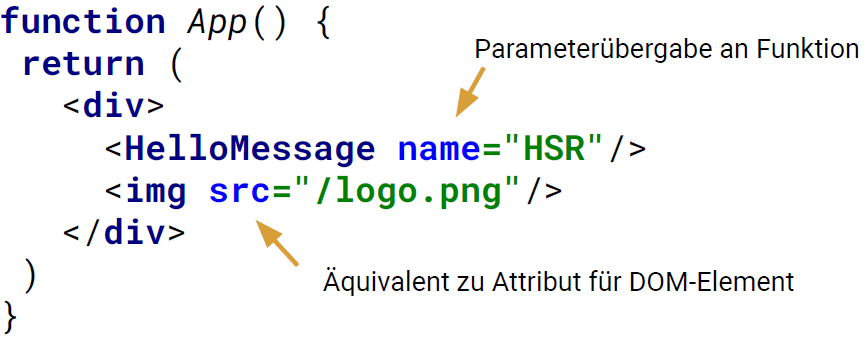
\includegraphics[width=0.6\linewidth]{img/react_component.png}

\subsection{JavaScript XML}
React verwendet JSX (blau), eine Erweiterung von JavaScript (gelb).
Überall wo JSX verwendet wird, muss $react$ importiert werden.\\
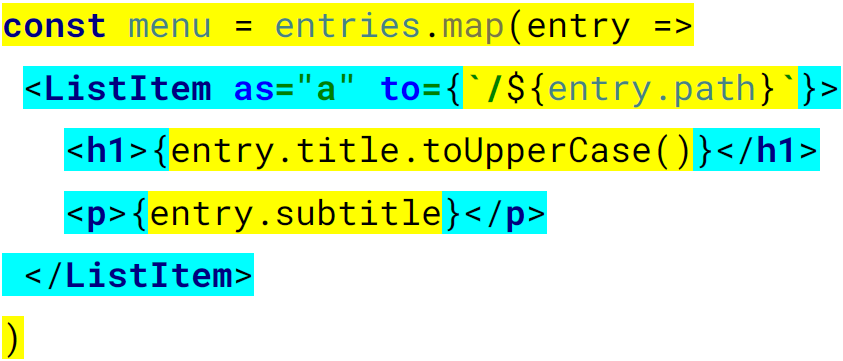
\includegraphics[width=0.6\linewidth]{img/react_jsx.png}\\
\textbf{Styles:} werden nicht als Strings sondern als Object angegeben.

\subsubsection{Conditionals}
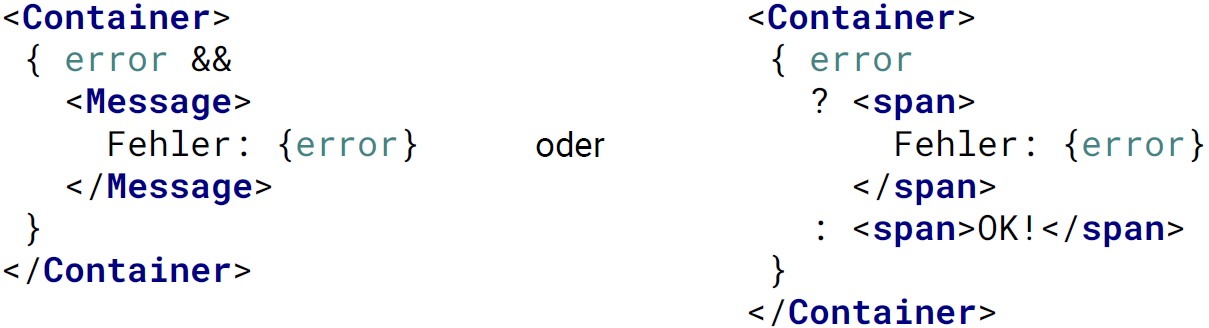
\includegraphics[width=0.7\linewidth]{img/react_jsx_conditionals.png}

\subsubsection{Props}
Komponenten erhalten alle Parameter/Properties als \textbf{props} Objekt.
\begin{itemize}
    \item $this.props$ bei Klassen
    \item Bei Funktionen als Parameter
    \item Immer \textbf{read-only}
\end{itemize}

\subsubsection{Rendering und Mounting}
\textbf{Mounting:} nötig um Komponenten auf Webseite anzuzeigen. \textit{ReactDOM.render}
\begin{lstlisting}
ReactDOM.render(
    <App/>
    document.getElementById('root')
)
\end{lstlisting}

\subsection{React State}
React-Klassenkomponenten können einen veränderbaren Zustand haben.
Der \textbf{state} einer Komponente ist immer privat.
Ändert der State, wird auch die Komponente aktualisiert.
\begin{lstlisting}
class Counter extends React.Component {
    state = { counter: 0 }
    // ...
}
\end{lstlisting}

\subsubsection{Event Handler}
\begin{lstlisting}
const increment = () => {
    this.setState({counter: this.state.counter + 1})
} // ...
<button onClick={this.increment}>
\end{lstlisting}

\subsection{Reconciliation}
\begin{enumerate}
    \item React Komponenten werden als virtueller DOM gerendert
    \item Wird der \textbf{state} geändert, erstellt React einen virtuellen DOM
    \item Alter und neuer DOM werden verglichen
    \item Erst dann werden geänderte DOM-Knoten im Browser erstellt
\end{enumerate}

\subsection{Formulare}
\subsubsection{Input Handling}
\begin{lstlisting}
<form onSubmit={this.handleSubmit}>
<input value={this.state.username}
        onChange={this.handleUsernameChange} //...
</form>
handleUsernameChange = (event) => {
    this.setState({username: event.target.value});
};
handleSubmit = (event) => {
    event.preventDefault();
    //...
}
\end{lstlisting}

\subsection{Komponenten Lifecycle}
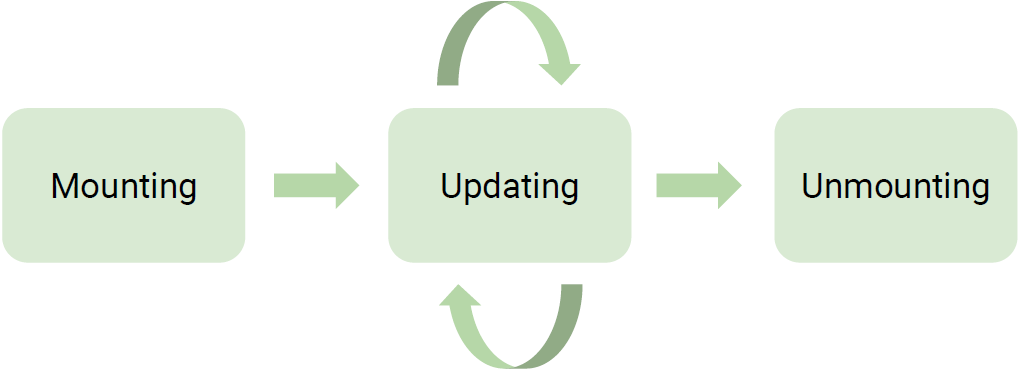
\includegraphics[width=0.7\linewidth]{img/react_lifecycle.png}
\subsubsection{Mounting}
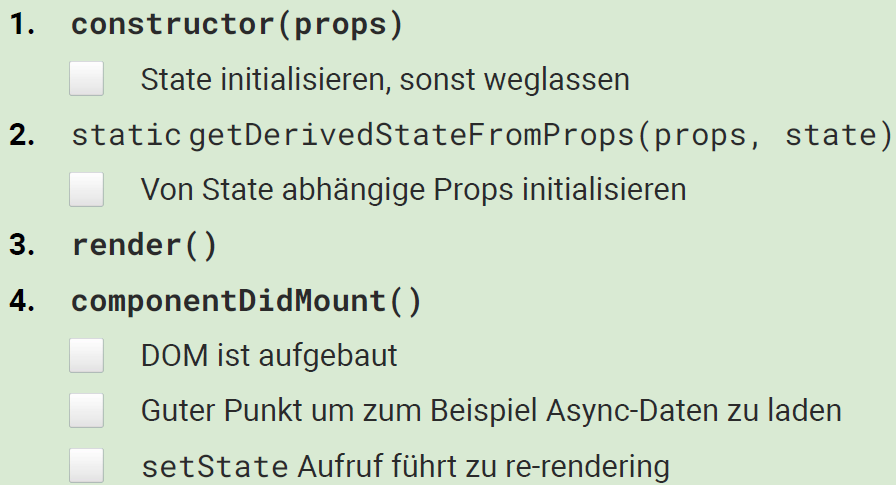
\includegraphics[width=0.7\linewidth]{img/react_mounting.png}

\subsubsection{Updating}
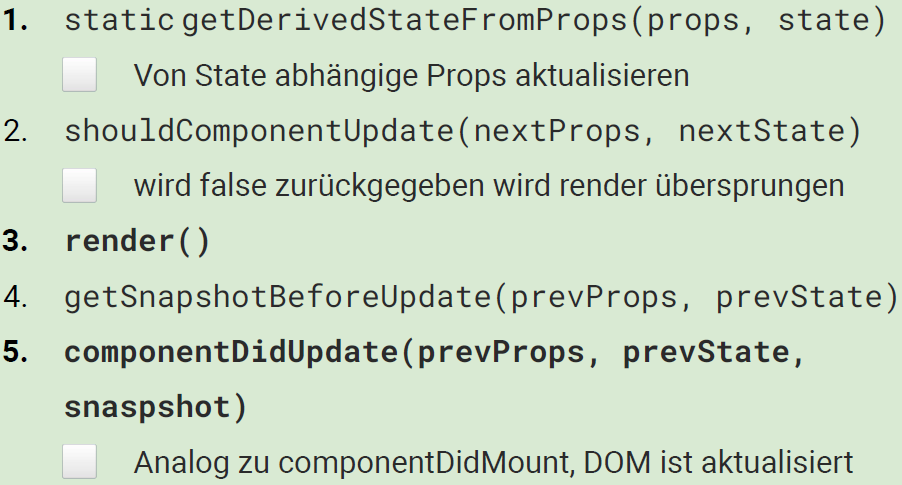
\includegraphics[width=0.7\linewidth]{img/react_updating.png}

\subsubsection{Unmounting}
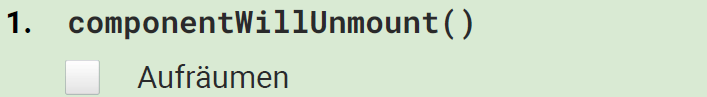
\includegraphics[width=0.6\linewidth]{img/react_unmounting.png}

\subsubsection{Error Handling}
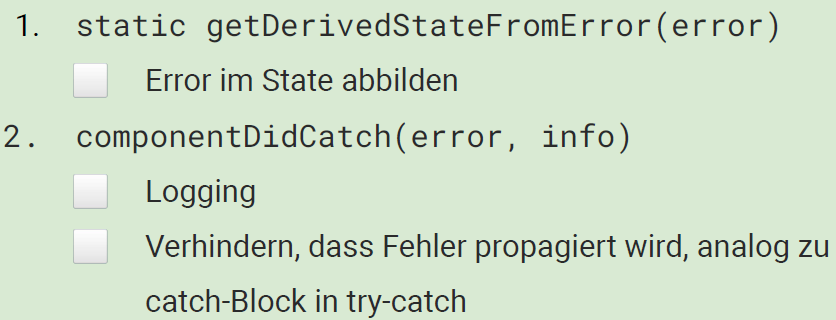
\includegraphics[width=0.7\linewidth]{img/react_error_handling.png}

\subsection{React Router}
\begin{itemize}
    \item Komponentenbibliothek
    \item Komponenten anzeigen oder verstecken abhängig von der URL
    \item Für React Web und React Native
\end{itemize}

\subsubsection{Router Komponenten}
\begin{lstlisting}
<Router>
\end{lstlisting}
Alle Routen müssen Teil des Routers sein, typischerweise nahe der Root-Komponente
\begin{lstlisting}
<Route exact path="/" component={Home} />
\end{lstlisting}
Home-Komponente wird nur gerendert, wenn der path (exakt) matcht.
Mehrere Route Elemente können gleichzeitig aktiv sein.
\begin{lstlisting}
<Link to="/">Home</Link>
\end{lstlisting}
App-interne Links, welche nicht wie \textless a \textgreater die Seite neu laden.
\begin{lstlisting}
<Redirect to="/somewhere/else">
\end{lstlisting}
Wird ausgeführt, sobald gerendert.

\subsection{Hooks}
\textbf{Problem von Lifecycle Methoden}
Zusammengehörender Code ist auf mehrere Methoden verteilt (Mount/Unmount).\\
\textbf{Problem von Klassen-State}
State ist über verschiedene Methoden verteilt\\
\textbf{Fazit:}
\begin{itemize}
    \item Lifecycle und State ohne Klassen machen react verständlicher
    \item Klassen sind weiterhin unterstützt
    \item Hooks erlauben, Logik mit Zustand einfacher wiederzuverwenden
\end{itemize}

\subsubsection{State Hook}
\begin{lstlisting}
function Counter() {
    const [count, setCount] = useState(0);
    // button => setCount(count + 1)
    return( <p>{count}</p> );
}
\end{lstlisting}
\textbf{Mehrere State-Variablen:} useState Aufrufe müssen immer in derselben Reihenfolge gemacht werden.

\subsubsection{Effect Hook}
\begin{lstlisting}
useEffect(() => {
    // Mount stuff
    return () => {
        // Unmount stuff
    }
}, [] /* <= Dependencies */);
\end{lstlisting}

\subsection{Flow}
\begin{itemize}
    \item Erweitert JavaScript um Typenannotationen
    \item Typ-Annotation im Code Typ-Inferenz für lokale Definitionen
    \item Generics, Maybe-Types, Union and Intersection-Types
\end{itemize}

\subsection{TypeScript und React}
\begin{itemize}
    \item Mehr Typensicherheit in React-Komponenten
    \item Props und State lassen sich typisieren
\end{itemize}
\textbf{Vorteil gegenüber Flow:}
\begin{itemize}
    \item Vollwertige Programmiersprache
    \item Besser unterstützt von Libraries und IDEs
    \item TypeScript Fehler müssen korrigiert werden
\end{itemize}

\subsection{React Context}
Ermöglicht es, Props für alle Unterkomponenten zur Verfügung zu stellen. (Theme Variablen)
\begin{lstlisting}
// provider
const c = React.createContext(themes.light);
const theme = useContext(c); // consumer
\end{lstlisting}

\subsection{Redux}
Library für Statemanagement (Repräsentation / Veränderung / Benachrichtigung).
State wird als Tree (immutable) von Objekten dargestellt.
Veränderung am Tree führt durch den Reducer zu einem neuen Tree t+1 (funktionale Programmierung).
State wird im \textbf{Store} verwaltet.

\subsubsection{Actions}
Benötigt um Stateänderungen zu machen.
Wird an den Store gesendet / dispatched.
Action ist eine reine Beschreibung der Action.
\begin{lstlisting}
{type: 'TRANSFER', amount: 100 }
\end{lstlisting}

\subsubsection{Reducer}
Pure Funktionen, haben keine Seiteneffekte.
\begin{lstlisting}
function balance(state = 0, action) {
    switch (action.type) {
        case 'TRANSFER':
            return (state + action.amount);
        default:
            return state;
    }
}
\end{lstlisting}
\textbf{Reducer kombinieren:} Jeder Reducer erhält einen Teil des States, für den er zuständig ist.
Resultat wird in einem neuen State-Objekt kombiniert.
\begin{lstlisting}
function rootReducer(state = {}, action) {
    return {
        balance: balance(state.balance, action),
        transactions: transactions(state.transactions, action)
    }
}
// Hilfsfunktion combineReducers:
const rootReducer = combineReducers({
    balance, transactions
});
\end{lstlisting}

\subsubsection{Store erstellen}
\begin{lstlisting}
const store = createStore(rootReducer);
\end{lstlisting}
Mit dem root-Reducer kann der Store erstellt werden.
In Kombination mit React führt das zu einem re-rendering der Komponenten.

\subsection{React \textless 3 Redux}
\textbf{Redux mit React verbinden:}
\begin{lstlisting}
const mapStateToProps = (state) => {
    return {
        transactions: state.transactions
    }
}
const mapDispatchToProps = {
    fetchTransactions
}
export default connect(mapStateToProps, mapDispatchToProps)(Component);

// Root Komponente
const store = createStore(
    rootReducer, applyMiddleware(thunkMiddleware));
render(
    <Provider store={store}>
        <App />
    </Provider>
    document.getElementById('root')
)
\end{lstlisting}
\textit{mapStateToProps:} erhält State und kann daraus Props ableiten.\\
Die Komponente bekommt auch die \textit{dispatch} Methode des Stores als Prop.
Das Resultat von \textit{connect} ist eine React-Komponente die mit dem Store verbunden ist.\\
Store muss der Root-Komponente mitgegeben werden.\\
\textit{thunkMiddleware:} Erlaubt es, anstelle eines Objektes eine Funktion zu dispatchen (benötigt für asynchrone Actions).

\subsubsection{Thunk Actions}
\begin{lstlisting}
function fetchTransactions(token) {
    return (dispatch, getState) => {
        dispatch({type: "FETCH_TRANSACTIONS_STARTED"});
        api.getTransactions(token)
            .then(({result: transactions}) => {
                dispatch({type: "FETCH_TRANSACTIONS_SUCCEEDED", transactions});
            })
    };
}
\end{lstlisting}

\subsubsection{Selectors}
Getter bei den Reducern, die einen Subtree des Stores zurückgeben.
Wissen über den Aufbau des State-Trees bleibt bei den Reducern.

    \end{multicols*}
\end{document}

























